\chapter{Mechanical characteristics}

\begin{ZubaxSimpleTable}{Mechanical characteristics}{| l | c | c | c | X | c |}
    Parameter       & Grosso  & Piccino  & Nudo  & Note                                & Unit \\
    Mass            & 228     & 128      & 62    & Cables and propellers not included     & g \\
    IP Protection   & 54      & 54       & 54    & Liquid damage protection is achieved 
                                                   by conformal \mbox{coating} of the PCB &   \\
\end{ZubaxSimpleTable}

The drawing \ref{fig:characteristics_connectors_placement} documents the placement of connectors and status LEDs on all variants of Zubax Sadulli.

\begin{figure}[!hbt]
    \centerline{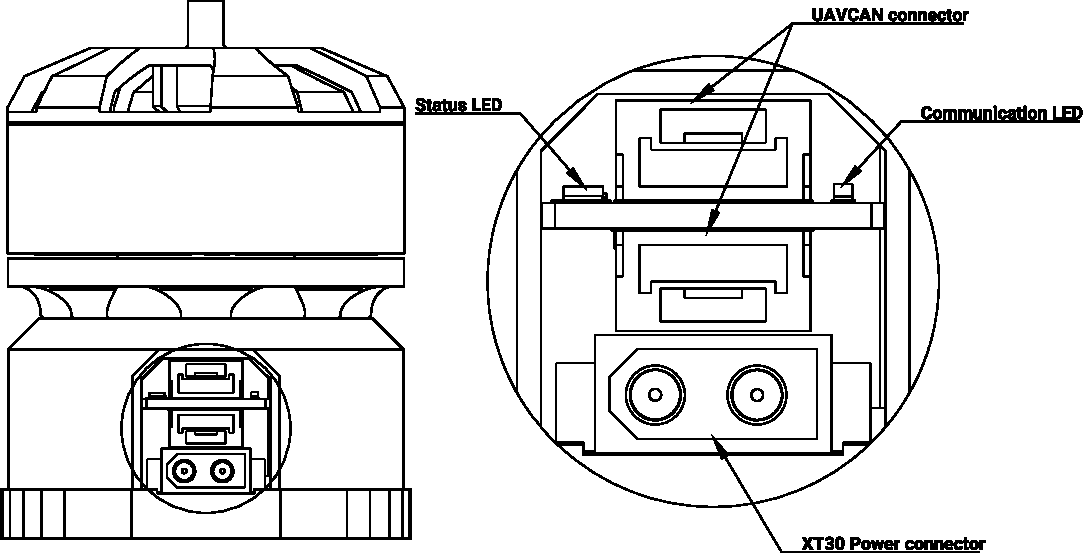
\includegraphics[width=0.8\textwidth]{figures/connectors_leds}}
    \caption{Connectors and LEDs drawing\label{fig:characteristics_connectors_placement}}
\end{figure}

\section{Mounting pattern}

All versions of Zubax Sadulli share the same mounting pattern. 
It is specified in the drawing \ref{fig:characteristics_mounting_pattern}. All linear dimensions are in mm.

\begin{figure}[!hbt]
    \centerline{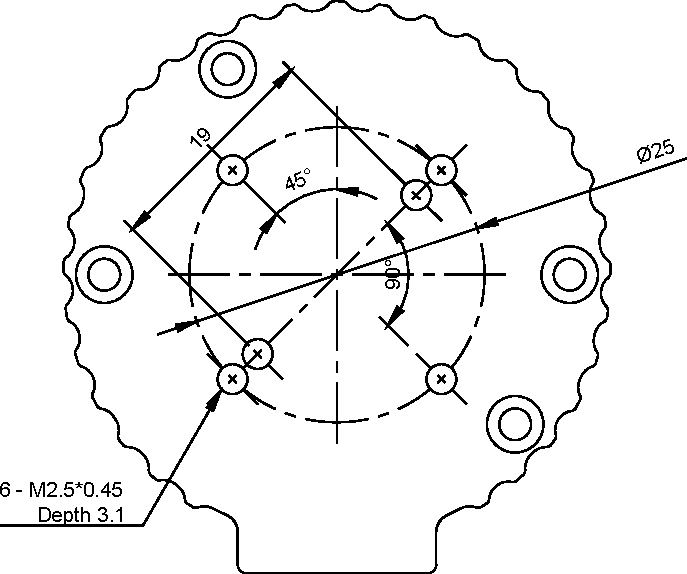
\includegraphics[width=0.5\textwidth]{figures/mounting_pattern}}
    \caption{Mounting pattern\label{fig:characteristics_mounting_pattern}}
\end{figure}

\newpage

\section{Sadulli nudo drawing}
All linear dimensions are in mm.

\begin{figure}[!hbt]
    \centerline{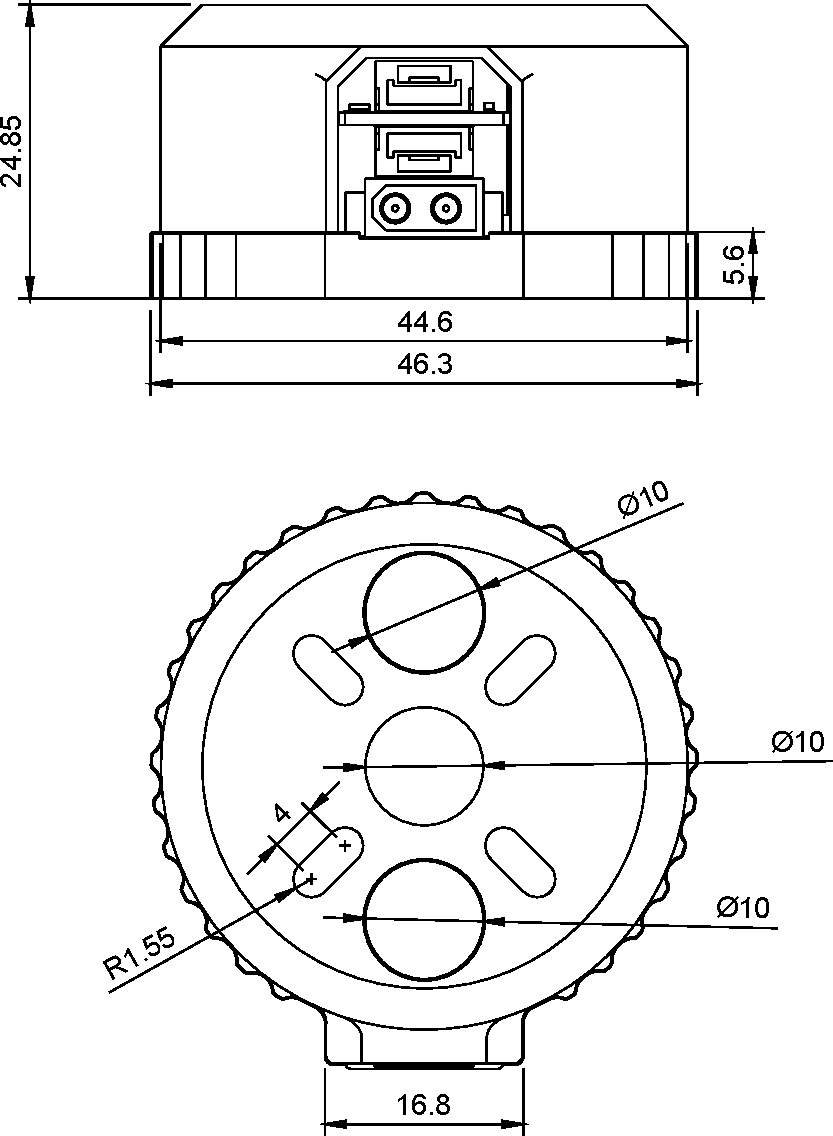
\includegraphics[width=0.6\textwidth]{figures/sadulli_nudo}}
    \caption{Sadulli Nudo drawing}
\end{figure}

\newpage

\section{Sadulli Piccino drawing}
All linear dimensions are in mm. Propeller not shown.

\begin{figure}[!hbt]
    \centerline{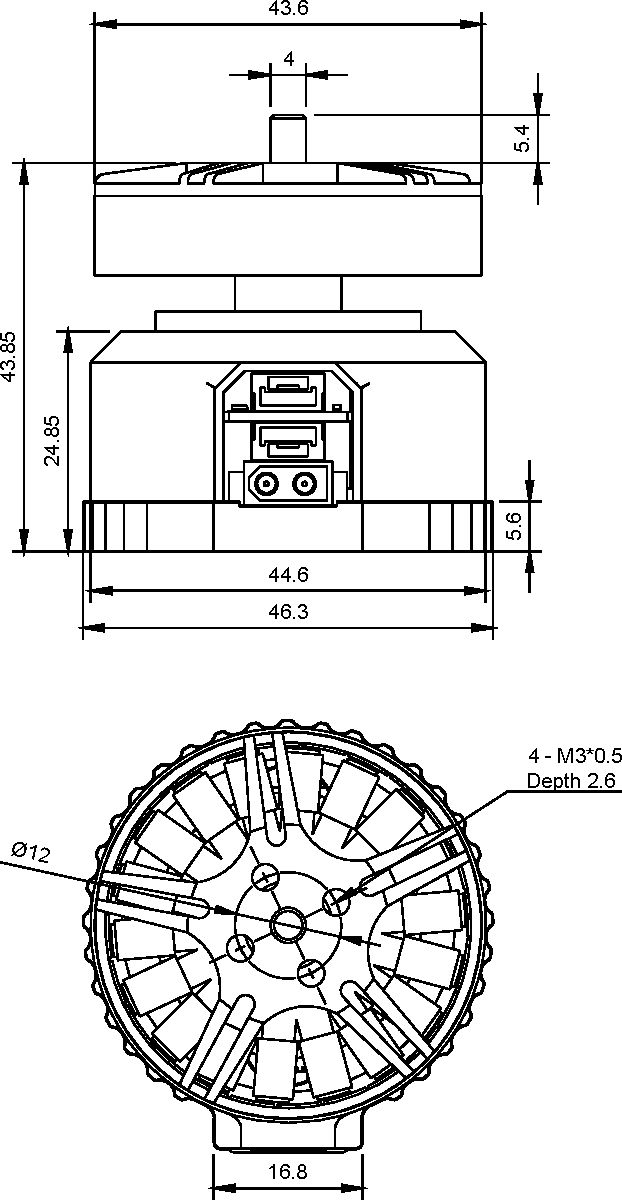
\includegraphics[width=0.6\textwidth]{figures/sadulli_piccino}}
    \caption{Sadulli Piccino drawing}
\end{figure}

\newpage

\section{Sadulli Grosso drawing}
All linear dimensions are in mm. Propeller not shown.

\begin{figure}[!hbt]
    \centerline{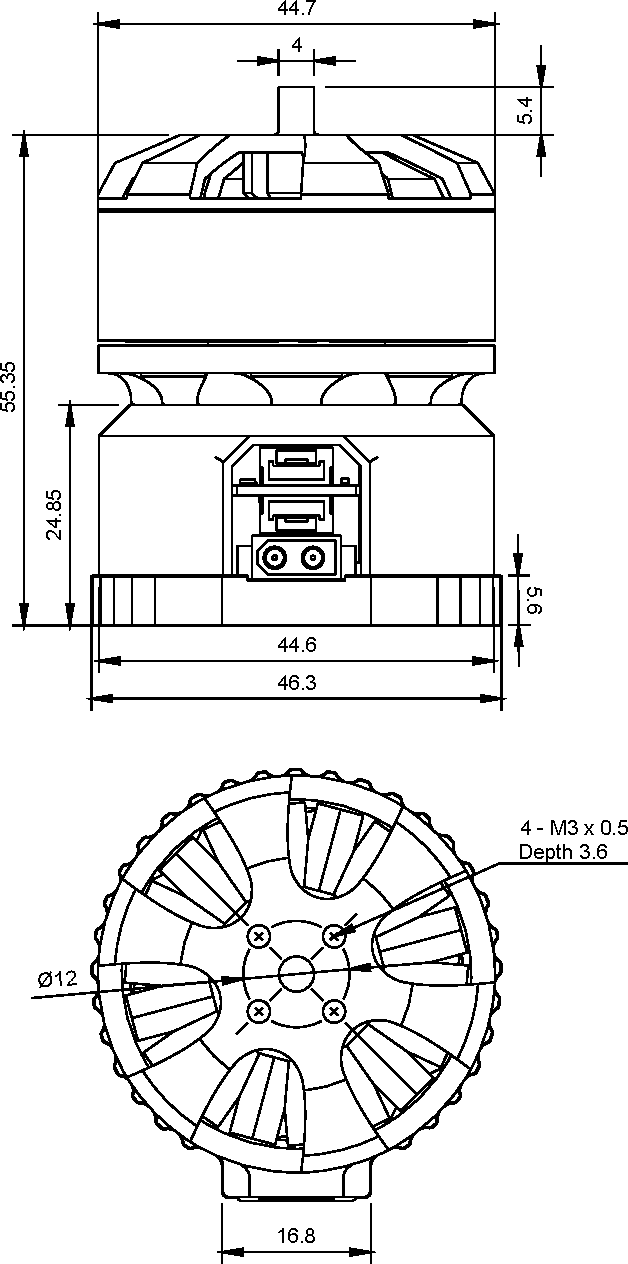
\includegraphics[width=0.6\textwidth]{figures/sadulli_grosso}}
    \caption{Sadulli Grosso drawing}
\end{figure}
